\documentclass{amsart}
\usepackage{master}
\begin{document}
\author{Lectures by Henry Horton\\
Notes by Jackson Van Dyke}
\thanks{All error introduced are my own.}
\title{An introduction to symplectic geometry.}
\maketitle

\section{Linear symplectic geometry}

\begin{defn}
A \emph{linear symplectic form} on a finite dimensional\footnote{We focus on finite dimensional
symplectic geometry. One can of course
do infinite dimensional symplectic geometry, only this can look a bit different.}
vector space $V$ is a bilinear
form $\om: V\times V\fromto \RR$ such that
\begin{enumerate}
\item $\om$ is skew-symmetric:
\begin{equation}
\om\left( u , v \right) = -\om\left( v , u \right)
\end{equation}
\item $\om$ is non-degenerate
\begin{equation}
\forall v\in V, \om\left( u , v \right) = 0
\implies u = 0
\end{equation}
\end{enumerate}
A vector space $\left( V , \om \right)$ is called a symplectic vector space.
\end{defn}

\begin{rmk}
The non-degenerate condition is equivalent to the map:
\begin{equation}
\begin{cd}
V\arrow{r}{\tilde \om}&
\dual{V} \\
w\arrow[mapsto]{r}&
\left( \tilde w: v\mapsto \om\left( u , v \right) \right)
\end{cd}
\end{equation}
being an isomorphism.
\end{rmk}

\begin{exm}
The space $\RR^{2n}$ admits a standard symplectic form
\begin{equation}
\om_{\text{std}} = 
\begin{pmatrix}
0 & I \\ -I & 0
\end{pmatrix}
\end{equation}
In the standard basis $\left\{ e_1, \cdots , e_{2n} \right\}$.
This can be written as a $2$-form:
\begin{equation}
\om_{\text{std}} = \sum_{k = 1}^n
\d{e_k} \ext \d{e_{k + n}}
\end{equation}
\end{exm}

\begin{exm}
Two vector spaces $\left( V_1 , \om_1 \right)$ and $\left( V_2 , \om_2 \right)$ are symplectomorphic if
there exists a linear isomorphism 
$T:V_1 \fromto V_2$ such that $T^* \om_2 = \om_1$.
Here
\begin{equation}
\left( T^* \om_2 \right) \left( u , v \right) = \om_2\left( Tu , Tv \right)
\end{equation}
\end{exm}

\begin{thm}
Any symplectic vector space $\left( V , \om  \right)$ admits a symplectic basis
\begin{equation}
\left\{ x_1 , \cdots , x_n , y_1 , \cdots , y_n \right\}
\end{equation} 
such that
\begin{align}
\om\left( x_j , y_k \right) = \dd_{jk}
&&
\om\left( x_i , x_j \right) = 0
\end{align}
\end{thm}

\begin{proof}
This is somehow like the Gram-Schmidt process.
Pick $x_1\in V$ nonzero. 
Since this is non-degenerate, there must be some $y_1\in V$ such that
$\om\left( x_1 , y_1 \right)\neq 0$. Now rescale $y_1$ to get $\om\left( x_1 , y_1 \right) = 1$.
Now let $V_1 = \Span\left( x_1 , y_1 \right)$. 
Then take the symplectic complement:
\begin{equation}
V_1^\om = 
\left\{ u\in V \st 
\forall v\in V_1,
\om\left( u , v \right) = 0 \right\}
\end{equation}
Then the claim is the following:
\begin{clm}
$V = V_1 \dsum V_1^\om$ 
\end{clm}
\begin{wrn}
This is not true in general.
\end{wrn}
Let $u\in V$ and write
$a = \om\left( u , x_1 \right)$ and
$b = \om\left( u , y_1 \right)$.
Then 
\begin{equation}
u = \ubr{\left( b x_1 - a y_1 \right)}{\in V_1} + 
\ubr{\left( u - b x_1 + a y_1 \right)}{\in V_1^\om}
\end{equation}

Now suppose $u\in V_1 \cap V_1^\om$ which implies $u = a x_1 + b y_1$
which implies $0 = \om\left( u , x_1 \right) = -b$
and $0 = \om\left( u , y_1 \right) = a$ which means $u = 0$.
Together this implies the claimed decomposition.

Now we can see that $\om$ restricts to 
$V_1^\om$ as a symplectic form, so repeat this process for $V_1^\om$. 
Since $V$ is finite dimensional, this will eventually stop.
\end{proof}

\begin{cor}
If $\left( V , \om \right)$ is a symplectic vector space, then
there exists $n$ such that
$\dim\left( V \right)= 2n$.
Furthermore, $\left( V , \om \right)$ is symplectomorphic to 
$\left( \RR^{2n} , \om_{\std} \right)$ via
\begin{align}
x_k\mapsto e_k
&&
y_k \mapsto e_{n + k}
\end{align}
\end{cor}

\section{Symplectic manifolds}

\begin{defn}
Let $M$ be a smooth manifold. Then a \emph{symplectic form} on $M$ is a 
$2$-form $\om\in \Om^2\left( M \right)$ such that
\begin{enumerate}
\item $\om$ is non-degenerate, that is, 
$\om_p: T_p M \times T_p M \fromto \RR$
is non-degenerate for all $p\in M$.
\item $\om$ is closed ($\d{\om} = 0$)
\end{enumerate}
\end{defn}

\begin{rmk}
\begin{enumerate}
\item Nondegeneracy gives a bundle isomorphism
\begin{equation}
\tilde \om : TM \fromto T^*M
\end{equation}
The point is that even though this is always an isomorphism (for example by choosing
a Riemannian metric) with a symplectic manifold, $\tilde \om$ gives a differently 
flavored identification.
\item Each tangent space is a symplectic vector space, so since these have to be 
even dimensional, so does the manifold.
\item Nondegeneracy is also equivalent to $\om^{\ext n}$ being a volume form.
Therefore a symplectic manifold always comes with an orientation.
\item Because $\om$ is closed it defines a de Rham cohomology class
$\om \in H^2\left( M ; \RR \right)$. 
Because we're orientable and nondegenerate, we get that if $M$ is closed (compact, 
boundaryless) then $\left[ \om \right] \neq 0$.
This means there is no exact symplectic form for closed $M$. 
However if $M$ is noncompact, $\om$ can be exact, and this is a nice thing to study. 
In fact we can explicitly write:
\begin{equation}
\om_\std = 
-d \left( \sum_{k = 1}^n e_{k + n} d e_{k} \right)
\end{equation}
\end{enumerate}
\end{rmk}

\begin{exm}
$\RR^{2n}$ is of course still a symplectic manifold.
\end{exm}

\begin{exm}
Consider the two-sphere:
\begin{equation}
S^2 = \left\{ p\in \RR^3
\norm{p} = 1\right\}
\end{equation}
Now we can write the tangent space explicitly as:
\begin{equation}
TS^2 = \left\{ p_1 v\in \RR^3 \st \norm{p} = 1, p\cdot v = 0 \right\}
\end{equation}
and define
\begin{equation}
\om_p\left( u, v \right) = p\cdot \left( u\times v \right)
\end{equation}
where $\times $ is just the cross-product in $\RR^3$. 
Then this is in fact a symplectic form.
To see this is nondegenerate, we can notice that
$\om_p\left( u , u\times p \right)= 1$. 
$\om$ is closed because $S^2$ is two-dimensional and $d\om\in \Om^3\left( S^2 \right)$.

Note that the $2$-sphere is the only symplectic sphere. 
That is, $S^{2n}$ admits no symplectic form for $n  > 1$.
This is because the second cohomology is zero for all such $S^{2n}$.
\end{exm}

\begin{exm}
If $\Sigma_g$ is a compact orientable surface of genus $g$, and $\om$ is any area form, it is certainly
non-degenerate, and for the same reason as for the sphere, it is closed.
\end{exm}

\begin{exm}
If $Q$ is a smooth $n$-dimensional manifold, 
consider local coordinates $\left( q_1 , \cdots , q_n , p_1 , \cdots , p_n \right)$
for $T^*Q$. We have a $1$-form
\begin{equation}
\lam = 
\sum_{k = 1}^n p_k d q_k
\end{equation}
and therefore a $2$-form $\om = -d \lam$. 
If we think of $\al \in \Om^1\left( Q \right)$ as a map $\al: Q\fromto T^* Q$,
then $\lam$ is characterized by $\al^* \lam = \al$. 
This is often called the tautological $1$-form.
$\left( T^* Q , \om \right)$ is symplectic.
\end{exm}

\begin{exm}
We can always take products of symplectic manifolds. 
If $\left( M , \om_M \right)$ and $\left( N , \om_N \right)$ are symplectic, 
then $\left( M \times N , -\om_M\times \om_N  \right)$ is symplectic.
Note that $\om_M\times \om_N$ is also a symplectic form, but having the sign is better
because of the relationship with symplectomorphisms.
\end{exm}

\begin{defn}
Two symplectic manifolds $\left( M , \om_M \right)$ and $\left( N , \om_N \right)$
are symplectomorphic if there exists a diffeomorphism $\phi:M\fromto N$ such that
$\phi^* \om_N = \om_M$. 
\end{defn}

\begin{thm}[Darboux]
Every point $p\in M$ in a symplectic manifold $\left( M , \om \right)$ has a neighborhood
$U$ such that $\left( I , \restr{\om}{U} \right)$ is symplectomorphic to 
$\left( \RR^{2n} , \om_\std \right)$.
\end{thm}

\begin{rmk}
In Riemannian geometry, the analogous result certainly does not hold.
Riemannian geometry has local invariants like curvature (and maybe some global invariants too)
but the point is that symplectic manifolds have only global invariants.
\end{rmk}

\section{Hamiltonian vector fields}

Recall gradient vector fields in Riemannian geometry.
Let $H:M\fromto \RR$ be a function.
Then a metric $g$ induces an isomorphism $\tilde g : TM \fromto T^*M$
and $\tilde g: \Gamma\left( TM \right) \fromto \Gamma\left( T^*M \right)$
and then $\grad\left( H \right) = \tilde g^{-1}\left( dH \right)$.
We then have an analogous construction defined by
\begin{equation}
X_H = \tilde \om^{-1}\left( dH \right)
\end{equation}
Just as $\grad H$ is orthogonal to level surfaces of $H$,
$X_H$ is always tangent to level surfaces.
Just like the gradient flow we have a Hamiltonian flow. 
The one-parameter semigroup of diffeomorphisms 
generated by $X_H$, $\phi_t^H$ is called the \emph{Hamiltonian flow} of $H$. 

\begin{exm}
Let's consider $\left( \RR^2 , dx \ext dy \right)$ and the Hamiltonian
$H\left( x , y \right)= x^2 + y^2$. 
Then this yields $X_H = \left( 2y , -2x \right)$ and then $\phi_t^H$ 
rotates counter-clockwise about the origin by $t$ radians. 
\end{exm}

\begin{exm}
On $\left( S^2 , d\theta \ext dz  \right)$ define $H\left( \theta , z \right) = z$ 
to be the height. Then $X_h = \p / \p \theta$, so we have
$\phi_t^H\left( \theta , z \right) = \left( \theta  + t , z \right)$ as in \cref{fig:sphere_hamiltonian}
\begin{figure}
\centering
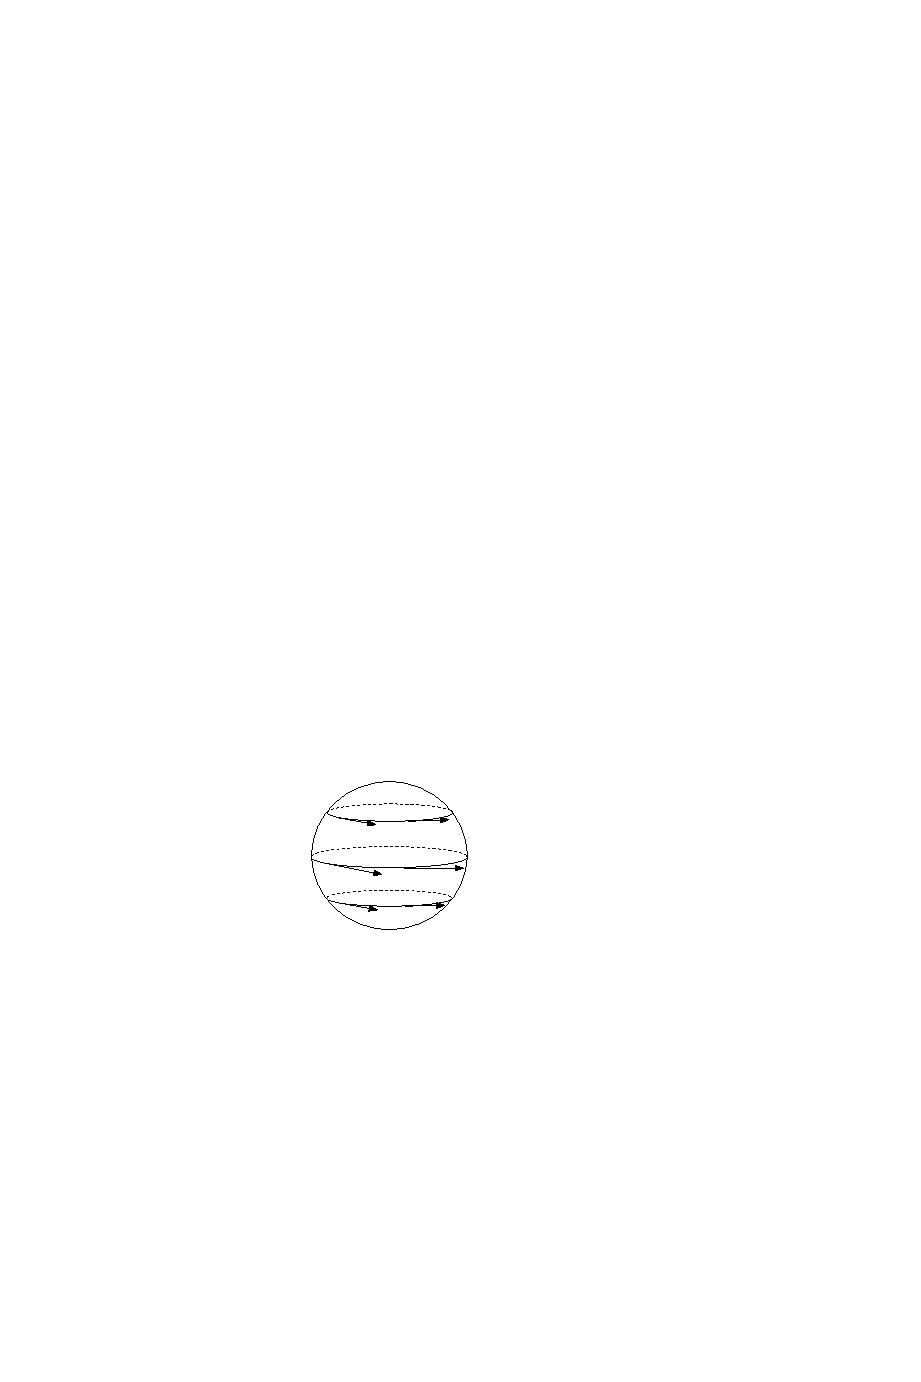
\includegraphics[width=0.2\textwidth]{sphere_hamiltonian}
\caption{Hamiltonian flow on $S^2$ where $H$ is the height function.}
\label{fig:sphere_hamiltonian}
\end{figure}
\end{exm}

\section{Almost-complex structures}

\begin{defn}
Let $M$ be a smooth manifold, then an almost-complex structure on $M$ is a bundle endomorphism
$J:TM \fromto TM$ such that $J^2 = -\id$.
The pair $\left( M , J \right)$ is called an almost-complex manifold.
\end{defn}

\begin{rmk}
A proper complex manifold has holomorphic coordinate charts.
\end{rmk}

Let $\cJ\left( M \right)$ denote the space of all almost complex structures on $M$.
If $\left( M , \om \right)$ is symplectic, we say that $J\in \cJ\left( M \right)$
is \emph{tamed} by $\om$ if $\om\left( v , Jv \right) > 0$
for all $p\in M$ and $v\in T_pM$. 
This is like saying complex lines are positively oriented with respect to the symplectic form.

$J\in \cJ\left( M \right)$ is called compatible with $\om$ if it is tamed by $\om$ and
$J$ gives a symplectomorphism on each tangent space, that is, 
for all $p\in M$ and all $u,v\in T_p M$, we have
$\om_p\left( Ju , Jv \right) = \om_p\left( u , v \right)$. 
We write $\cJ\left( M , \om \right)$ for the space of $\om$-compatible almost complex structures.

\begin{thm}
$\cJ\left( M , \om \right)$ is nonempty and contractible for any symplectic manifold $\left( M , \om \right)$.
\end{thm}

We won't go through it here, but the proof establishes a one-to-one correspondence between
Riemannian metrics $M$ and compatible almost complex structure.
That is for every Riemannian metric, we get a unique $J\in \cJ\left( M , \om \right)$, then the space of 
Riemannian metrics is convex and contractible, so this is done.

Recall that a complex manifold $M$ of complex dimension $n$
is a smooth manifold equipped with an atlas such that the local coordinate neighborhoods are 
identified with $\CC^n$. 
So it must be even dimensional, and the transition functions for overlaps
are holomorphic functions.

\begin{clm}
If $M$ is a complex manifold, then in charts, we get
\begin{equation}
J_0 = 
\begin{pmatrix}
0 & -I \\ I & 0
\end{pmatrix}
\end{equation}
for coordinates $\left( x_1 , \cdots , x_n , y_1 , \cdots , y_n \right)$,
so these local almost complex structures paste together to make a global almost complex structure.
\end{clm}

The converse is not true, 
and if $J\in \cJ\left( M \right)$ induces a complex structure then it's called integrable.

A K\"ahler manifold is a triple $\left( M , J , \om \right)$ where $\left( M , \om \right)$
is symplectic, and $J$ is a compatible almost complex structure.
$\om$ is called a K\"ahler form, and the K\"ahler metric is
\begin{equation}
g\left( u , v \right) = \om\left( u , Jv \right)
\end{equation}
So K\"ahler manifolds always have a Riemannian structure.

\begin{exm}
Our standard example $\left( \RR^{2n} , J_0 , \om_\std \right)$ is a K\"ahler manifold.
\end{exm}

\begin{exm}
Complex projective spaces $\CP^n$ are K\"ahler.
The K\"ahler form $\om_{\FS}$ is called the Fubini-Study form.
If $\phi: \CC^{n+1}\minus \left\{ 0 \right\} \fromto S^{2n + 1}$
which maps $z\mapsto z / \abs{z}$, 
then $w_\FS$ is the unique $2$-form on $\CP^n$ whose pullback under the projection
\begin{equation}
\CC^{n+1} \minus \left\{ 0 \right\} \fromto \CP^n
\end{equation}
is $\phi^*\left( \restr{\om_\std}{S^{2n+1}} \right)$.
\end{exm}

\begin{prop}
A complex submanifold of a K\"ahler manifold is K\"ahler.
The K\"ahler form of this submanifold is just the restriction.
\end{prop}

\begin{cor}
Smooth complex projective varieties\footnote{
These are smooth manifolds arising as a zero-set of some homogeneous polynomials.}
are K\"ahler.
\end{cor}

\begin{exm}
Any $K3$ surface is K\"ahler since it is a smooth complex projective variety.
\end{exm}

\end{document}
